%%% -*-LaTeX-*-

\chapter{Introduction}
\label{cha:introduction}

% A few sentences on the priming project

Interactions between the blood and artificial materials is an
important engineering problem. Artificial devices are commonly used to
treat cardiovascular diseases, and they must be designed to not
trigger immune responses in the bloodstream. However, current designs
are not sufficiently blood-compatible and patients with a
blood-contacting device must be placed on systemic anticoagulants to
reduce the risks of thrombosis and embolism
\cite{Ratner1993,Ratner2007,Oprea13}. %There's probably another
                                %transition sentence that needs to go
                                %here.
It is important to first know
how the blood clotting system is ``supposed'' to work before
understanding the problems that arise when an artificial device is
implanted into the bloodstream.
	
% 2. Contextualize rolling within blood clotting
% Process of clotting begins when agonists (vWF and collagen) are
% exposed on the ECs

\section{Overview of the clotting pathway}
\label{sec:overview-clotting}

\begin{figure}
  \centering
  % \documentclass{article}
% \usepackage{tikz}
% \usetikzlibrary{backgrounds,fit,positioning}

% \begin{document}

\begin{tikzpicture}[
  node text/.style={
    align=center,
    draw, very thick,
    fill=white,
    rounded corners,
    inner xsep=10pt,
    inner ysep=7pt,
    minimum height=13mm,
  },
  connect/.style={shorten <=5pt, shorten >=5pt, thick},
  background/.style={rounded corners, inner xsep=10pt, inner ysep=10pt, draw, dashed,
    thick},
  ]
  
  \node[node text] (roll)
  {\begin{minipage}{.5\linewidth}
      \underline{Rolling}
      \begin{itemize}
        \setlength\itemsep{-.3em}
      \item transient contacts
      \item hydrodynamic vs. bond forces
      \item fast receptors trigger intracellular pathways
      \end{itemize}
    \end{minipage}
  };
  \node[node text] (actv) [below=of roll]
  {\begin{minipage}{.5\linewidth}
      \underline{Activation}
      \begin{itemize}
        \setlength\itemsep{-.3em}
      \item intracellular signaling
      \item release soluble agonists
      \item activate integrins for aggregation
      \end{itemize}
    \end{minipage}
  }
  edge [<-, connect] (roll);
  \node[node text] (aggr) [below=of actv]
  {\begin{minipage}{.5\linewidth}
      \underline{Aggregation}
      \begin{itemize}
        \setlength\itemsep{-.3em}
      \item cohesion among platelets
      \item adhesion to vessel wall
      \end{itemize}
    \end{minipage}
  }
  edge [<-, connect] (actv);
  \node[node text] (thrb) [below=2cm of aggr]
  {\begin{minipage}{.5\linewidth}
      \underline{Thrombin Formation}
      \begin{itemize}
        \setlength\itemsep{-.3em}
      \item plasma-phase reactions
      \item many coagulation factors involved
      \item prothrombin converted to thrombin
      \end{itemize}
    \end{minipage}
  }
  edge [<-, thick, shorten <=28pt, shorten >= 15pt] (aggr);
  \node[node text] (fibr) [below=of thrb]
  {\begin{minipage}{.5\linewidth}
      \underline{Fibrin Gelation}
      \begin{itemize}
        \setlength\itemsep{-.3em}
      \item thrombin converts fibrinogen to fibrin
      \item stabilize the clot
      \end{itemize}
    \end{minipage}
  }
  edge [<-, connect] (thrb);

  \begin{scope}[on background layer]
    \node [fill=lightgray, fit=(roll) (aggr), background,
    label=above:\textbf{Activation and Aggregation}] {};
    \node [fill=gray, fit=(thrb) (fibr), background,
    label=above:\textbf{Coagulation}] {};
  \end{scope}
\end{tikzpicture}
% \end{document}


  \caption[The clotting pathway]{Sketch of the major processes in the
    clotting pathway}
  \label{fig:clot-path}
\end{figure}

There are two major processes in the blood clotting pathway: platelet
activation/adhesion and coagulation. In platelet adhesion and
activation, chemical platelet agonists are exposed on the vessel wall
and released into the fluid, signaling platelets to begin clot
formation and adhere to the vessel wall. As activated platelets begin
to aggregate, extracellular chemical reactions begin to occur both in
the blood and on platelet surfaces ultimately resulting in the
production of thrombin, and the formation of a fibrin
gel. Collectively these two processes are called coagulation
\cite{Fogelson2015}. 

The process of platelet activation is mediated through
intracellular chemical pathways. When a platelet binds with agonists,
activation pathways are triggered which result in a suite of
activation responses: degranulation (i.e. release of ADP and other
soluble agonists), thromboxane A2 (TxA2) synthesis, activation and
recruitment of \ITA{IIb}\ITB{3} receptors, exposure of
phosphatidylserine (PS), and---after adhesion to a vessel
wall---platelet spreading \cite{Bye2016}.

Coagulation broadly refers to the extracellular chemical reaction
network that produces thrombin. Thrombin is a soluble platelet
agonist, and so mediates further activation of platelets throughout
the blood. Thrombin is also the chemical which initiates the process
of fibrin gelation, by cleaving fibrinogen to form fibrin
monomers. Finally these fibrin monomers can polymerize to form a
fibrin gel, which stabilizes the blood clot \cite{Fogelson2015}. These
two processes do not occur in sequence, but in parallel with abundant
cross-talk between them. Coagulation can upregulate activation through
the production of thrombin, activation upregulates coagulation by
exposing PS on platelet surfaces, and platelet adhesion can
downregulate coagulation by blocking tissue factor and slowing the
pathways required to form thrombin \cite{Kuharsky2001}. 


\subsection{Platelet adhesion to an injury and aggregate formation}
\label{sec:platelet-adhesion}

In order for a platelet aggregate to form, two processes need to
occur: platelet adhesion to the vessel wall, and cohesion among
platelets. In normal hemostasis, adhesion is facilitated by two
surface-immobilized proteins: collagen embedded in the sub-endothelial
matrix, and von Willebrand factor (vWF) which can either be bound to
collagen in the SE matrix or expressed by endothelial cells when
activated \cite{Fogelson2015}. Platelets in the blood can roll along
these proteins using fast-forming and fast-breaking bonds, and through
these contacts activation pathways within the platelet are
triggered. As a platelet is activated, receptors on the platelet
surface are activated which can mediate stable, long lasting bonds
with vWF and collagen \cite{Bye2016,Li2010,Fogelson2015,Qiu2015}. 
%% (see refs in Fogelson and Neeves, 2015, pp. 384 \& 390).
		
% Platelets bind to these agonists with fast receptors first (GP1b and
% GPVI), and then later with slow receptors (\alpha{IIb} \beta{3} and
% \alpha{2} \beta{1}).
Platelets constitutively express GP1b and GPVI receptors for vWF and
collagen respectively. These receptors have fast binding and unbinding
kinetics, and are therefore able to form bonds with their
surface-immobilized ligands while the platelet is moving past the
surface in the blood. When these bonds form and are stretched beyond
their rest length, they exert a force in opposition to the flow and
slow the platelet down. Therefore the motion of a platelet along a
wall with immobilized agonists is a function of the biochemical
interactions of receptors and ligands as well as the fluid forces
exerted on the platelet.
		
% The fast receptors trigger intracellular signaling cascades that
% result in platelet activation and activation of the slow receptors.
These receptors are more than simple physical links between the
platelet and surface. When they are bound with a ligand, they initiate
intracellular signaling cascades that are responsible for triggering
release of intracellular calcium and activating
phosphatidylinositide-3-kinase (PI3K) which are two crucial events in
platelet activation \cite{Bye2016,Du2007,Senis2014}. These activation
pathways ultimately terminate in a suite of responses that are
collectively called ``platelet activation,'' including granule
secretion, TxA2 synthesis, cytoskeletal rearrangements, and activation
of integrins \ITA{IIb}\ITB{3} and \ITA{2}\ITB{1}. These integrins are
receptors for fibrinogen/vWF and collagen, respectively. They are
constitutively expressed on the surface of the platelet, but on
unactivated platelets they exist mostly in their low-affinity
conformation and undergo a conformational change to their
high-affinity conformation after platelet activation
\cite{Qiu2015,Shattil1998,Shattil2010}.
		
In general, integrins form a large group of transmembrane receptors
that are primarily involved in the adhesion of cells to extracellular
matrix (ECM) \cite{Giancotti1999}. They have a large extracellular
domain---called the ectodomain---with a hinge. In the low affinity
conformation, the ectodomain is bent at the hinge and the ligand
binding domain is at least partially blocked. When switching from
low-affinity to high-affinity conformations the integrin ectodomain
extends at the hinge to reveal the ligand binding site
\cite{Campbell2011,Qiu2015,Shattil1998}. Once integrins are bound and
in their high-affinity conformation, they can activate signal
transduction pathways to initiate the formation of clusters of
integrins that mediate firm adhesion of a cell to ECM along with other
responses \cite{Hynes2002,Li2010,Shattil1998,Shattil2010}.

\subsection{Secondary activation and platelet cohesion}
\label{sec:second-wave-activ}

An important result of platelet activation is the release of secondary
mediators of platelet activation TxA2 and ADP \cite{Bye2016}. These
are soluble platelet agonists which enter the blood and activate
platelets in the bulk flow, forming a positive feedback loop where
activated platelets release chemical signals that trigger more
platelets to activate. \emph{(Can I say something about a wave of activating
chemical seen in previous coagulation models by Aaron and his
students?)} Platelets that are activated in the blood must
then be recruited to the growing clot by either adhering to collagen
or vWF exposed on the wall, or by cohering to an existing platelet
aggregate. 

Cohesion among platelets is mediated by vWF and fibrinogen---the
precursor to fibrin monomers \cite{Fogelson2015}. As mentioned before,
vWF is bound by the GP1b and \ITA{IIb}\ITB{3} receptors on the
platelet surface, and fibrinogen is bound by \ITA{IIb}\ITB{3}. Both of
these molecules circulate within the blood plasma, and activated
platelets can bind to them. Once a platelet is adhered to the wall, it
can capture both vWF and fibrinogen, which then act as a cross-bridge
to which other platelets within the blood can cohere.

\subsection{Coagulation: thrombin generation and fibrin gelation}
\label{sec:coagulation}

There are two closely related subprocesses in coagulation: thrombin
generation through the tissue factor (TF) pathway, and fibrin gel
formation. Thrombin is produced on the external face of platelet
plasma membranes, and is both a potent activator of platelets
\cite{Heemskerk2002,Heemskerk2013} and catalyzes fibrinogen conversion
to fibrin monomers (try to find sources for this, search Mendeley).

%% Is this section necessary?

The TF pathway is initiated when TF embedded in the SEM is exposed to
the bloodstream. Tissue factor can complex with an active enzyme
present in the blood plasma to initiate a cascade of enzyme activation
in the plasma, and on the surface of activated platelets. When
platelets are strongly activated, they expose phosphatidylserine (PS)
on the blood-facing side of their plasma membrane, to which
coagulation factors can bind and catalyze activation of other
membrane-bound proteins. These surface-mediated reactions are an
important part \emph{((this is a bit weasley and vague))} of the coagulation
pathway \cite{Fogelson1998,Kuharsky2001}.
	
% Once platelets are activated, they can bind firmly to the wall,
% release soluble platelet agonists which causes a platelet aggregate to
% form, and release thrombin which results in the formation of a fibrin
% gel which ultimately stabilizes a clot.

% 3. Description of cell rolling, a single cell interacting with the surface
% Should mention margination in here somewhere.
% Cell rolling is the important first part of the process of platelet
% activation. There are three main insoluble platelet agonists: vWF,
% collagen, and fibrinogen. Two important constitutively active platelet
% receptors are GP1b (binds to vWF) and GPVI (binds to collagen). These
% receptors have fast association and dissociation and mediate platelet
% rolling along a vessel wall.
% There are also constitutively expressed integrins \alpha{IIb}
% \beta{3} and \alpha{2} \beta{1}, however they are in their
% low-affinity conformation.

% 1. Description of the priming project

% Why is hemocompatibility important?

% \section{Platelet rolling}
% \label{sec:platelet-rolling}

\section{Description of the priming project}
\label{sec:priming-project}

Cardiovascular disease is one of the leading causes of death in the
U.S, and a common treatment for these diseases is to implant medical
devices into the blood stream. For example, stents (an expandable
solid mesh) are often used to treat stenotic arteries. However, the
introduction of a foreign material into the blood stream will cause
thrombosis unless the material is treated somehow, and while these
devices have been effective in saving lives, they are still far from
perfect. Patients with these implanted devices still must be placed on
anticoagulants, as they have a higher risk of a thrombotic event even
when the device is functional and surgery is successful
\cite{Cannegieter1994}.

% What has been done so far in hemocompatibility research, and what is
% Vlado's group trying to add?
Most hemocompatibility studies focus on local interactions and effects
of the material on platelets. However recent work
\cite{Corum2011,Corum2012} has shown that nonlocal effects are also
important in understanding platelet interactions with implanted
biomaterials. In particular they have shown that platelet interactions
with immobilized agonists may not cause the platelets to adhere at the
site of interaction, but can nonetheless prime them for downstream
adhesion and full activation.

\begin{figure}
  \centering
  \begin{tikzpicture}[scale=.65]
  \tikzstyle{every node}=[font=\small]
  \pgftext{\includegraphics[width=\textwidth]{blood-vessel}}
  \draw[very thick, ->] (-3, 2.6) -- node[fill=white] {flow direction} +(5,.35);
  \draw[thick, ->] (-3.5, -3.5) node[below] {Native vessel} -- ++(0, 1);
  \draw[thick, ->] (1, -3.3) node [below] {Artificial vessel} -- ++(0, 1);
  \draw[thick, ->] (-1, -4) node[below] {Anastomoses} .. controls (-1, -2) .. +(-1.4, 3);
  \draw[thick, ->] (-.8, -4) .. controls (-.8, -2) and (0, -1) .. +(2.55, 3.5);
\end{tikzpicture}

  \caption{Cross-section of a blood vessel}
  \label{fig:blood-vessel}
\end{figure}

One possible example of this in a vascular graft is shown in Figure
\ref{fig:blood-vessel}. At either end of the implanted device, native
tissue must be joined with the artificial device. At these points
along the vessel wall the tissue is inflamed and anastomotic, which
could expose platelet agonists on the surface of the
wall. Additionally the increased shear rate in the stenotic regions
could act as a platelet agonist through a phenomenon known as
shear-induced platelet activation
\cite{Fogelson2015,Kroll96,Shankaran2003}. Therefore while platelets
may not bind to a single inflamed region of the vessel, the upstream
region may prime platelets for adhesion, and then more readily bind to
the downstream inflamed region. It is also possible that the inflamed
tissue or the biomaterial may not cause platelets to bind locally, but
nonetheless partially activate platelets and cause them to adhere
downstream somewhere in the circulation.
		
% Describe experimental setup, ongoing experiments, etc
In order to investigate nonlocal effects of priming, Dr. Hlady's group
has designed a microfluidic assay with two regions printed with
platelet agonists (see Figure \ref{fig:flow-chamber})
\cite{Corum2012}. The upstream agonist region is called the priming
region, and the downstream region with agonist is called the capture
region. In the priming region, platelets that are close to the
agonist-printed surface of the flow chamber may have transient
contacts with the agonist, initiating activation pathways within the
platelet. Some platelets may firmly adhere in this priming region, but
many will not and instead reenter the flow and get washed downstream
to the capture region. Once they reach the capture region, the
platelets which contacted the agonist in the priming region will have
more active integrin on their surfaces \cite{Corum2012}, more
phosphatidylserine exposed (unpublished data), and probably heightened
levels of intracellular activating chemicals like Ca$^{++}$. That is,
they will be ``primed'' to adhere with the capture region, and
therefore adhere with a greater frequency than unprimed platelets.

\begin{figure}
  \centering
  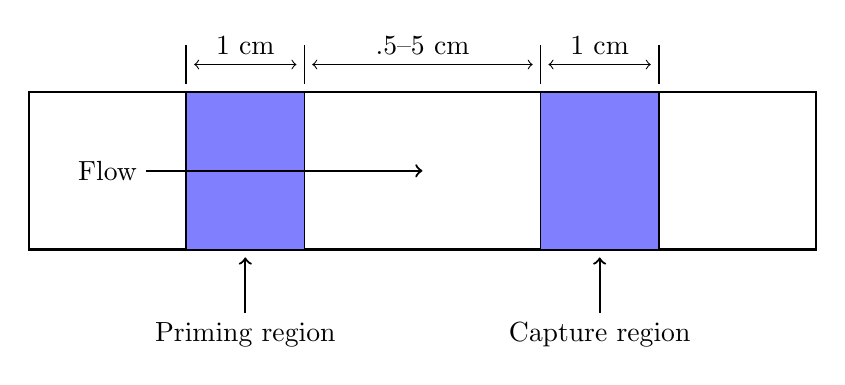
\begin{tikzpicture}
  \draw[thick] (-5, -1) rectangle (5, 1);
  \filldraw[semithick, fill=blue!50] (-3, -1) rectangle (-1.5, 1);
  \filldraw[semithick, fill=blue!50] (1.5, -1) rectangle (3, 1);
  \draw[thick, ->] (-4, 0) node[fill=white] {Flow} -- (0, 0);
  \draw[thick, ->] (-2.25, -1.8) node[below] {Priming region} -- ++(0, .7);
  \draw[thick, ->] (2.25, -1.8) node[below] {Capture region} -- ++(0,
  .7);
  \draw[semithick] (-3, 1.1) -- +(0, .5);
  \draw[semithick] (-1.5, 1.1) -- +(0, .5);
  \draw[semithick] (1.5, 1.1) -- +(0, .5);
  \draw[semithick] (3, 1.1) -- +(0, .5);
  \draw[<->] (-2.9, 1.35) -- node[midway, above] {1 cm} +(1.3, 0);
  \draw[<->] (1.6, 1.35) -- node[midway, above] {1 cm} +(1.3, 0);
  \draw[<->] (-1.4, 1.35) -- node[midway, above] {$.5$--$5$ cm}(1.4,
  1.35);
\end{tikzpicture}

  \caption{Flow chamber}
  \label{fig:flow-chamber}
\end{figure}

In previous research, Dr. Hlady's group has found that all 3
immobilized platelet agonists tested (vWF, collagen, and fibrinogen)
in the upstream region increased adhesion of platelets in the capture
region relative to a nonreactive control
\cite{Corum2012,Eichinger2016}. Recent unpublished work has shown
similar results when the upstream agonist printing is replaced by a
stenotic region with higher wall shear rates (unpublished data). In
addition, flow cytometry has revealed that platelets in blood which
has been perfused over surface-immobilized agonists express higher
levels of P-selectin (a marker for degranulation), high-affinity
\ITA{IIb}\ITB{3}, exposed PS, and lysosomal glycoprotein (another
marker of degranulation) (see \cite{Corum2012,Eichinger2016} and
unpublished data).

\section{Existing cell rolling models}
\label{sec:exist-cell-roll}

A large body of work has been published on the subject of cell rolling
and adhesion, including mathematical models of cell rolling
\cite{Pospieszalska2009,Sundd2011}. However most of the modeling work
has been done on leukocyte rolling on an agonist-coated surface, and
relatively less work has been done on platelet rolling.

\subsection{Adhesive dynamics (AD) models}
\label{sec:adhesive-dynamics}

Adhesive dynamics (AD) is a common modeling framework for leukocytes,
and the first AD model was published in 1992 by Hammer \& Apte
\cite{Hammer1992}. The Hammer and Apte paper provides a good example
to describe the AD models in general. It is convenient to view the
more recent models as modifications of this fundamental model. They
model a leukocyte as a rigid sphere, with rigid microvilli protruding
normally from the surface of the cell. Receptors are located only at
the tips of these microvilli (multiple receptors can occupy a single
microvillus), and can bind to ligand binding sites which are uniformly
distributed along a flat wall. The positions and bound state of each
receptor is tracked throughout the simulation. Binding and unbinding
of receptors is modeled with a stochastic process with
length-dependent rates given by the Dembo model \cite{Dembo1988}:
\begin{align}
  \label{eq:dembo-on}
  k_\tn{on} \left(L_\tn{sep}\right)
  &= k_\tn{on}^0 \exp \left( -\frac{\sigma_\tn{ts} (L_\tn{sep} -
    \lambda)^2}{2\boltzmann \temp} \right) \\
  \label{eq:dembo-off}
  k_\tn{off} \left(L_\tn{sep}\right)
  &= k_\tn{off}^0 \exp \left( \frac{(\sigma - \sigma_\tn{ts})
    (L_\tn{sep} - \lambda)^2}{2 \boltzmann \temp} \right).
\end{align}
where $\lambda$ is the equilibrium separation distance,
$\boltzmann\temp$ is the thermal energy, $\sigma$ is the spring
constant, and $\sigma_\tn{ts}$ is the transition state spring
constant.

The movement of the leukocyte is determined by balancing hydrodynamic
forces and various chemical forces. The hydrodynamic forces are found
by assuming that the fluid surrounding the leukocyte is a Newtonian
fluid with $\Reynolds = 0$ at the revelent length and time scales of
the problem, and the fluid is moving in a shear flow. Under this set
of assumptions, there is a linear relationship between the drag force
$\forceVec$ on the cell and the velocity $\velVec$: $\forceVec =
\resMatrix \velVec$. The chemical forces on the cell are split up into
5 different forces: bond forces between the cell and the surface, van
der Waals forces, gravitational body force, electrostatic force, and
steric stabilization force.

\subsubsection{Extensions of AD}
\label{sec:extensions-ad}

Many extensions and adaptations of the AD model have been made since
its publication. \cite{King2001} uses the AD framework to model the
dynamics and interactions of multiple cells rolling on a surface at
once. In \cite{Bhatia2003}, Bhatia, King, and Hammer model leukocyte
rolling with two classes of receptors: fast binding and unbinding
selectins (P-selectin--sLe\textsuperscript{x}), and slow binding and
unbinding integrins (\ITB{2}-integrin--ICAM-1). They plot the effect
of modulating the selectin and integrin ligand surface densities by
creating state diagrams which characterize the cell rolling behavior
in different regions of this 2D parameter space. They showed the
effect of neutrophil activation on these state diagrams by increasing
the $k_\tn{on, integrin}^0$ value.

A platelet adhesive dynamics (PAD) model is developed in
\cite{Mody2008a} and \cite{Mody2008b}, which is used to model the
aggregation of non-spherical platelets in a shear flow through binding
with vWF. The PAD model was later adapted to model the dynamics of
platelet rolling on a vWF-coated wall, with collisions between rolling
platelets and free-flowing platelets \cite{Wang2013}.

Adhesive dynamics models are detailed and expensive, because they
explicitly model individual receptors on the cell surface, and many of
them require solving Stokes' equations at every time step. Of the
receptors involved in rolling of platelets and leukocytes, there can
be between thousands to tens of thousands of a specific receptor on
the cell surface. In order to simulate the cell motion near the
surface, these models require calculating all the forces generated by
links between the cell and the surface, all forces arising from
nonspecific chemical interactions, and all drag and shear forces
exerted by the moving fluid on the cell. In the simplest possible
case---a rigid sphere---this involves evaluating a $6 \times 6$
resistance matrix as a function of the height $\height$ of the cell
and then inverting it. For non-spherical geometries, Stokes' equations
must be solved at every time step to generate the resistance matrix,
greatly increasing the computational cost.

\subsection{Semi-analytic rolling models}
\label{sec:semi-analytic}

In contrast to the expensive AD models, semi-analytic models save on
computational cost by tracking bond and receptor densities in the
cell-substrate contact region instead of tracking every bond
individually \cite{Pospieszalska2009}. An early example of this comes
from T\"{o}zeren and Ley \cite{Tozeren1992}. % I need to read a bit
                                % more about this first before going
                                % into the other rolling models
